\documentclass[10pt,a4paper]{article}
\usepackage[utf8]{inputenc}
\usepackage[spanish,es-tabla]{babel}
\usepackage{url}
\usepackage{natbib}
\usepackage{hyperref}
\usepackage{amsmath}
\usepackage{amsfonts}
\usepackage{amssymb}
\usepackage{graphicx}
\usepackage{float}
\usepackage{lipsum}
\usepackage{multicol}
\usepackage{array}
\usepackage{booktabs}
\usepackage{xcolor}
\usepackage{tabularx}
\definecolor{azul}{rgb}{0.0, 0.53, 0.74}
\usepackage[left=2.00cm, right=2.00cm, top=2.00cm, bottom=2.00cm]{geometry}

%%%%%%%%%%%%%%%%%%%%%%%%%%%%%%%%%%%%%%%%%%%%%%%%%%%%%%%%%%%%%%%%%%
\author{Autor}
\title{Título}

%%%%%%%%%%%%%%%%%%%%%%%%%%%%%%%%%%%%%%%%%%%%%%%%%%%%%%%%%%%%%%%%%%%%%%%%%

\begin{document}
	
	\begin{figure}[H]
		\raggedright
		
\includegraphics[scale=0.25]{LogoEsan.jpeg} \hfill 
	\end{figure}

%%%%%%%%%%%%%%%%%%%%%%%%%%%%%%%%%%%%%%%%%%%%%%%%%%%%%%%%%%%%%%%%%%%%%%%%%	
	\begin{center}
		{\Large \textbf{Implementación de un chatbot basado en Inteligencia Artificial generativa aplicado a la atención de clientes para la venta de programas de postgrado de una institución educativa}}\\
		\vspace{2mm}
		{\normalsize {Bolivar Leon, Sebastian Alonso}\\
		\vspace{7.5mm}

        Universidad ESAN. Facultad de Ingeniería. Ingeniería de Tecnología de Información y Sistemas.\\
	\end{center}

	\begin{center}
		\textcolor{azul}{\rule{150mm}{0.5mm}}
	\end{center}		
%%%%%%%%%%%%%%%%%%%%%%%%%%%%%%%%%%%%%%%%%%%%%%%%%%%%%%%%%%%%%%%%%%%%%%%%%%%

%%%%%%%%%%%%%%%%%%%%%%%%%%%%%%%%%%%%%%%%%%%%%%%%%%%%%%%%%%%%%%%%%%%%%%%%%%%	
%%%%%%%%%%%%%%%%%%%%%%%%%%%%%%%%%%%%%%%%%%%%%%%%%%%%%%%%%%%%%%%%%%%%%%%%%%%
	\section{Capitulo 1}
		    
%%%%%%%%%%%%%%%%%%%%%%%%%%%%%%%%%%%%%%%%%%%%%%%%%%%%%%%%%%%%%%%%%%%%%%%%%%%
	
	\subsection{Descripcion de la Realidad Problematica}
En los últimos años, la transformación digital ha impulsado cambios significativos en la manera en que las organizaciones interactúan con sus clientes. La aparición de tecnologías avanzadas, como la inteligencia artificial (IA), ha permitido a las empresas mejorar la eficiencia y efectividad en sus procesos, particularmente en la atención al cliente. Dentro de este marco, los chatbots han emergido como una de las herramientas más prometedoras para automatizar y optimizar la comunicación con los usuarios, mejorando tanto la velocidad de respuesta como la calidad de la atención.\\

Los chatbots, sistemas informáticos diseñados para imitar conversaciones humanas, están ganando terreno rápidamente en diversos sectores. Su implementación se ha acelerado debido a su capacidad de utilizar procesamiento de lenguaje natural (PLN) para comprender y responder a las consultas de los usuarios de manera eficiente. De acuerdo con Goasduff (2019), para 2022 más del 70\% de las empresas medianas y grandes habrán implementado chatbots en alguno de sus procesos, lo que destaca la relevancia de esta tecnología en el entorno empresarial moderno. Esto es particularmente significativo en sectores como el educativo, donde la atención personalizada es clave para captar y retener a los estudiantes, especialmente en programas de postgrado.\\

Los programas de postgrado suelen implicar un alto grado de especialización y, por lo tanto, requieren una atención al cliente que no solo sea eficiente, sino también precisa y personalizada. Los potenciales estudiantes buscan información detallada sobre los programas, desde los requisitos de admisión hasta los contenidos del curso y las oportunidades de financiamiento. Sin embargo, muchas instituciones educativas enfrentan desafíos en este ámbito debido a la falta de personal especializado, la sobrecarga de consultas o la incapacidad de brindar respuestas rápidas y oportunas. Este es un problema crítico, dado que una mala experiencia en la fase de consulta puede llevar a la pérdida de posibles estudiantes.\\

En este contexto, la implementación de un chatbot basado en IA generativa presenta una solución viable para mejorar la atención al cliente en las instituciones educativas que ofrecen programas de postgrado. Al utilizar tecnologías de procesamiento de lenguaje natural, los chatbots pueden proporcionar respuestas rápidas y precisas a las preguntas frecuentes de los estudiantes, al mismo tiempo que brindan una experiencia personalizada que se adapta a las necesidades individuales de cada usuario. Esto no solo reduce la carga de trabajo del personal de atención al cliente, sino que también mejora la experiencia del usuario, lo que puede resultar en un aumento de las inscripciones en los programas de postgrado.\\

Además, los chatbots son particularmente eficaces para gestionar interacciones repetitivas y de baja complejidad, como la respuesta a preguntas comunes sobre fechas límite, requisitos de admisión o estructura de los programas. Al automatizar estas tareas, las instituciones educativas pueden liberar recursos que se pueden destinar a la atención de consultas más complejas que requieren la intervención de personal especializado. Esto no solo mejora la eficiencia operativa, sino que también aumenta la satisfacción del cliente, ya que los estudiantes potenciales reciben respuestas rápidas y precisas sin tener que esperar largos periodos de tiempo.\\

A pesar de los beneficios potenciales de los chatbots, muchas instituciones educativas aún no han adoptado esta tecnología de manera integral. Una de las razones de esta reticencia es la percepción de que los chatbots no son capaces de manejar consultas complejas o de brindar un servicio al cliente verdaderamente personalizado. Sin embargo, los avances en inteligencia artificial, en particular en el campo de la IA generativa, han permitido el desarrollo de chatbots que son cada vez más capaces de imitar el lenguaje y la comunicación humana de manera natural y fluida.\\

De hecho, según Gartner (2017), la interacción entre humanos y máquinas está evolucionando rápidamente, y se espera que en el futuro la mayoría de las interacciones de servicio al cliente sean realizadas por sistemas de IA. Este cambio es impulsado no solo por la necesidad de mejorar la eficiencia operativa, sino también por las expectativas crecientes de los usuarios, en particular de los millennials, que valoran la rapidez, la conveniencia y la capacidad de acceder a información inmediata. En este sentido, la implementación de chatbots no solo responde a una necesidad interna de las instituciones educativas de mejorar sus procesos de atención al cliente, sino también a una demanda externa de los estudiantes que buscan una experiencia más rápida y personalizada.\\

Otra razón por la que la implementación de chatbots es crucial en las instituciones educativas es la creciente competencia en el mercado de los programas de postgrado. Con más instituciones ofreciendo programas especializados y con la globalización de la educación, las universidades y escuelas de negocios deben diferenciarse no solo por la calidad de sus programas, sino también por la calidad del servicio al cliente que brindan. Un chatbot basado en IA puede convertirse en una ventaja competitiva clave, al ofrecer una experiencia de consulta más eficiente y amigable para los potenciales estudiantes.\\

En términos de efectividad, los chatbots también son una herramienta poderosa para recopilar y analizar datos de los usuarios. Cada interacción con un chatbot genera información valiosa sobre las necesidades y expectativas de los estudiantes potenciales. Estos datos pueden ser utilizados por las instituciones educativas para mejorar sus estrategias de marketing, personalizar aún más sus programas y ajustar su oferta de acuerdo con las demandas del mercado. Además, el análisis de las interacciones puede ayudar a identificar patrones o áreas de mejora en el proceso de atención al cliente, permitiendo a las instituciones optimizar continuamente su servicio.\\

Un estudio de SAP Hybris (2019) resalta que los departamentos más beneficiados por la implementación de chatbots son los de servicio al cliente (72\%), ventas (45\%) y marketing (42\%). Este dato es particularmente relevante para las instituciones educativas que buscan mejorar su proceso de ventas y marketing de programas de postgrado. Los chatbots no solo pueden reducir los tiempos de respuesta y mejorar la satisfacción del cliente, sino que también pueden aumentar las tasas de conversión al proporcionar información clara y oportuna a los estudiantes potenciales.\\

En el ámbito nacional, la adopción de tecnologías basadas en inteligencia artificial ha ido en aumento, especialmente en sectores donde la necesidad de optimizar la atención al cliente es crucial. Huang \& Rust (2018) destacan que los chatbots son una herramienta común de IA que interactúa de manera natural con los usuarios, utilizando tanto texto como voz para manejar consultas diversas. En el caso de las instituciones educativas, el uso de chatbots puede ser particularmente eficaz para mejorar la atención al cliente en áreas como marketing, soporte técnico y, sobre todo, en la venta de programas de postgrado.\\

Sin embargo, a pesar de los beneficios mencionados, también es importante reconocer los desafíos asociados con la implementación de chatbots. Uno de los principales retos es garantizar que los chatbots sean capaces de manejar consultas complejas de manera efectiva. Si bien los avances en IA generativa han mejorado significativamente la capacidad de los chatbots para imitar conversaciones humanas, todavía existen limitaciones en su capacidad para resolver problemas más complejos que requieren juicio o intervención humana. Por lo tanto, es crucial que las instituciones educativas adopten un enfoque híbrido, donde los chatbots manejen consultas simples y repetitivas, y el personal especializado se enfoque en las interacciones más complejas.\\

Además, otro desafío importante es la integración de los chatbots en los sistemas existentes de las instituciones educativas. Para que un chatbot sea verdaderamente eficaz, debe estar integrado con las bases de datos y los sistemas de gestión de la institución, lo que permite una respuesta más precisa y personalizada. Este proceso de integración puede ser costoso y requerir una inversión significativa en infraestructura tecnológica. Sin embargo, los beneficios a largo plazo de una mayor eficiencia operativa y una mejor experiencia del cliente justifican esta inversión inicial.\\

Finalmente, la implementación de chatbots también plantea cuestiones éticas y de privacidad. Las instituciones educativas deben garantizar que los datos recopilados a través de las interacciones con los chatbots se manejen de manera segura y conforme a las regulaciones de protección de datos. Además, es importante que los usuarios sean conscientes de que están interactuando con un chatbot y no con un ser humano, para evitar confusiones o expectativas poco realistas.\\

La implementación de un chatbot basado en inteligencia artificial generativa en instituciones educativas que ofrecen programas de postgrado puede transformar significativamente el proceso de atención al cliente. Al mejorar la velocidad de respuesta, reducir la carga de trabajo del personal y ofrecer una experiencia más personalizada, los chatbots pueden aumentar las tasas de conversión y mejorar la satisfacción del cliente. No obstante, su implementación exitosa requiere un enfoque cuidadoso que considere tanto los beneficios como los desafíos asociados con esta tecnología emergente.\\

La institución educativa cuenta con programas de postgrado, agrupados por temáticas o procesos de negocio como Finanzas, Administración, Derecho, Operaciones y Tecnología de la Información. Cada una de ellas cuenta con un número de cursos, lo cual permite a los clientes lograr una especialización en las materias que requieran.\\

Durante un año lectivo se lanzan 10 campañas de ventas de cursos, que corresponden a los programas de postgrado. Estan campañas se realizan en diversos medios de comunicación, como redes sociales y correos electrónicos. Está a cargo del área de contact center hacer contacto con los clientes y responder a las consultas sobre los cursos a aperturarse, especializaciones, horarios, costos, profesores, modalidad de pagos y demás información que puede cerrar la venta de los cursos.\\

En la actualidad, se llega a captar entre 750 a 1, 000 clientes por campaña de programas de postgrado, pero hay una demanda no atendida de más del 100\%, siendo uno de los problemas las limitaciones del equipo de contact center en el tiempo dedicado a contestar las llamadas y consultas de los clientes.

		    
%%%%%%%%%%%%%%%%%%%%%%%%%%%%%%%%%%%%%%%%%%%%%%%%%%%%%%%%%%%%%%%%%%%%%%%%%%%
	\section{Formulacion del Problema}
		    
%%%%%%%%%%%%%%%%%%%%%%%%%%%%%%%%%%%%%%%%%%%%%%%%%%%%%%%%%%%%%%%%%%%%%%%%%%%
	\subsection{Problema General}

	La presente investigación responde a la pregunta formulada como problema  general: ¿De qué manera el uso de un Chatbot, mejora el proceso de venta de cursos de postgrado, específicamente en la atención de clientes?
 
%%%%%%%%%%%%%%%%%%%%%%%%%%%%%%%%%%%%%%%%%%%%%%%%%%%%%%%%%%%%%%%%%%%%%%%%%%

    \subsection{Problemas Especificos}
	Asimismo, como problemas específicos tenemos: ¿En qué medida el uso de  un Chatbot reduce el tiempo promedio de espera del cliente en el proceso de ventas  de cursos de postgrado?, ¿En qué medida el uso  de un Chatbot reduce el tiempo para dar una respuesta al cliente en el proceso de  ventas de cursos de postgrado?, ¿En qué medida  el uso de un Chatbot reduce el tiempo para generar una cotización en el proceso de  ventas de cursos de postgrado?

 		    
%%%%%%%%%%%%%%%%%%%%%%%%%%%%%%%%%%%%%%%%%%%%%%%%%%%%%%%%%%%%%%%%%%%%%%%%%%%
	\section{Objetivos de la Investigacion}
		    
%%%%%%%%%%%%%%%%%%%%%%%%%%%%%%%%%%%%%%%%%%%%%%%%%%%%%%%%%%%%%%%%%%%%%%%%%%%
	\subsection{Objetivo General}

	Se estableció como objetivo general de la presente investigación: Determinar que un Chatbot mejora el proceso de ventas de cursos de postgrado.

 
%%%%%%%%%%%%%%%%%%%%%%%%%%%%%%%%%%%%%%%%%%%%%%%%%%%%%%%%%%%%%%%%%%%%%%%%%%

    \subsection{Objetivos Especificos}
	Como objetivos específicos se planteó: Determinar que un Chatbot reduce el tiempo promedio de espera del cliente en el proceso de ventas de cursos de postgrado. Determinar que un Chatbot reduce el tiempo para dar una respuesta al cliente en el proceso de ventas de cursos de postgrado. Determinar que un Chatbot reduce el tiempo para generar una cotización en el proceso de ventas de cursos de postgrado.


 		    
%%%%%%%%%%%%%%%%%%%%%%%%%%%%%%%%%%%%%%%%%%%%%%%%%%%%%%%%%%%%%%%%%%%%%%%%%%%
	\section{Hipotesis}
		    
%%%%%%%%%%%%%%%%%%%%%%%%%%%%%%%%%%%%%%%%%%%%%%%%%%%%%%%%%%%%%%%%%%%%%%%%%%%
	\subsection{Hipotesis General}

	Como hipótesis general se establece que: Si se usa un Chatbot, entonces mejora el proceso de ventas de cursos de postgrado.

 
%%%%%%%%%%%%%%%%%%%%%%%%%%%%%%%%%%%%%%%%%%%%%%%%%%%%%%%%%%%%%%%%%%%%%%%%%%

    \subsection{Hipotesis Especificos}
	Asimismo como hipótesis específica se planteó que: Si se usa un Chatbot, entonces se reduce el tiempo promedio de espera del cliente en el proceso de ventas de cursos de postgrado. Si se usa un Chatbot, entonces reduce el tiempo para dar una respuesta al cliente en el proceso de ventas de cursos de postgrado. Si se usa un Chatbot, entonces reduce el tiempo para elaborar una cotización al cliente en el proceso de ventas de cursos de postgrado.

 		    
%%%%%%%%%%%%%%%%%%%%%%%%%%%%%%%%%%%%%%%%%%%%%%%%%%%%%%%%%%%%%%%%%%%%%%%%%%%
	\section{Justificacion de la Investigacion}
		    
%%%%%%%%%%%%%%%%%%%%%%%%%%%%%%%%%%%%%%%%%%%%%%%%%%%%%%%%%%%%%%%%%%%%%%%%%%%
	\subsection{Teorica}

	La investigación tiene como objetivo transformar el proceso de atención al cliente en la venta de cursos de postgrado mediante la implementación de un chatbot basado en inteligencia artificial. El uso de este chatbot permitirá ofrecer respuestas rápidas y personalizadas, optimizando la experiencia del cliente desde el primer contacto hasta la cotización final. Al aplicar metodologías ágiles, el estudio aporta un enfoque novedoso en el ámbito educativo, específicamente en la atención automatizada para la promoción de programas de postgrado. Los resultados serán aplicables a otras instituciones educativas con necesidades similares, proporcionando un marco de referencia para mejorar la competitividad en el mercado de la educación superior.

 
%%%%%%%%%%%%%%%%%%%%%%%%%%%%%%%%%%%%%%%%%%%%%%%%%%%%%%%%%%%%%%%%%%%%%%%%%%

    \subsection{Practica}
	La implementación del chatbot mejorará la eficiencia operativa del proceso de ventas de programas de postgrado, reduciendo tiempos de espera, agilizando respuestas y acelerando la generación de cotizaciones. Esto beneficiará directamente tanto a la institución educativa, que optimizará sus procesos y aumentará su competitividad, como a los potenciales estudiantes, quienes recibirán un servicio más rápido y eficiente. Además, este estudio proporcionará un modelo replicable para otras instituciones educativas que buscan automatizar sus procesos de ventas, reduciendo costos y mejorando la experiencia del cliente.

  
%%%%%%%%%%%%%%%%%%%%%%%%%%%%%%%%%%%%%%%%%%%%%%%%%%%%%%%%%%%%%%%%%%%%%%%%%%

    \subsection{Metodologia}
	Esta investigación aborda problemas clave en el proceso de ventas de cursos de postgrado, como los largos tiempos de espera, la demora en la respuesta al cliente y el tiempo necesario para generar cotizaciones. La automatización de estos procesos mediante el chatbot reducirá significativamente estos tiempos, mejorando la experiencia del cliente. Se utilizarán métodos cualitativos y cuantitativos, incluyendo encuestas a los potenciales clientes y análisis de los tiempos de respuesta actuales, para medir la eficacia del chatbot. Además, permitirá segmentar mejor a los prospectos, ofreciendo soluciones más personalizadas que optimizan los tiempos de atención y mejoren la calidad de la interacción en el proceso de ventas.

 %%%%%%%%%%%%%%%%%%%%%%%%%%%%%%%%%%%%%%%%%%%%%%%%%%%%%%%%%%%%%%%%%%%%%%%%%%%
	\section{Delimitación del Estudio}
		    
%%%%%%%%%%%%%%%%%%%%%%%%%%%%%%%%%%%%%%%%%%%%%%%%%%%%%%%%%%%%%%%%%%%%%%%%%%%
	\subsection{Espacial}

	El estudio se realizará en una institución de educación superior comercial, ubicada en el distrito de Santiago de Surco, con sede en la ciudad de Lima, Perú.

 
%%%%%%%%%%%%%%%%%%%%%%%%%%%%%%%%%%%%%%%%%%%%%%%%%%%%%%%%%%%%%%%%%%%%%%%%%%

    \subsection{Temporal}
	El estudio se llevará a cabo durante los meses de octubre del 2024 a diciembre del 2024.

  
%%%%%%%%%%%%%%%%%%%%%%%%%%%%%%%%%%%%%%%%%%%%%%%%%%%%%%%%%%%%%%%%%%%%%%%%%%

    \subsection{Conceptual}
	El estudio está delimitado al conocimiento de las herramientas chatbot y su uso para implementarlo y mejorar la atención de clientes en una institución de educación superior para la venta de cursos de postgrado: Programas de Especialización Ejecutiva, Diplomados, Maestrías y Doctorados. 

 %%%%%%%%%%%%%%%%%%%%%%%%%%%%%%%%%%%%%%%%%%%%%%%%%%%%%%%%%%%%%%%%%%%%%%%%%%%
	\section{Anexo}
		    
%%%%%%%%%%%%%%%%%%%%%%%%%%%%%%%%%%%%%%%%%%%%%%%%%%%%%%%%%%%%%%%%%%%%%%%%%%%
	\subsection{Árbol del problema}

	\begin{figure}[H]
		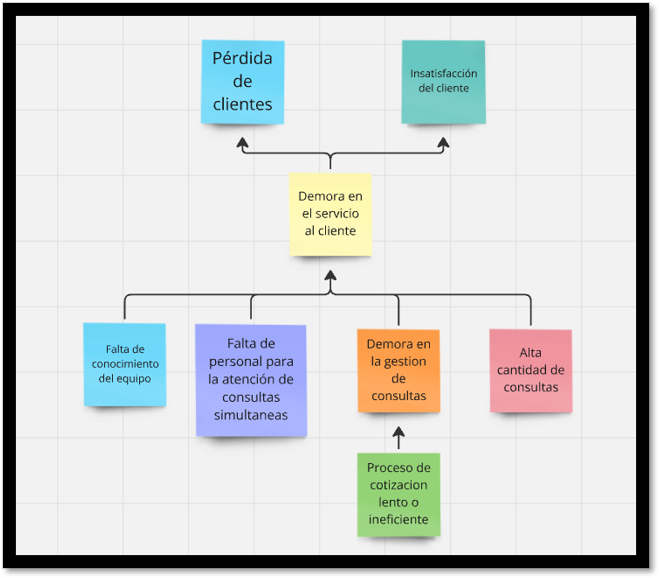
\includegraphics[scale=1]{ArbolProblema.png} \hfill 
	\end{figure}
 
%%%%%%%%%%%%%%%%%%%%%%%%%%%%%%%%%%%%%%%%%%%%%%%%%%%%%%%%%%%%%%%%%%%%%%%%%%

    \subsection{Árbol de objetivos}

	
	\begin{figure}[H]
		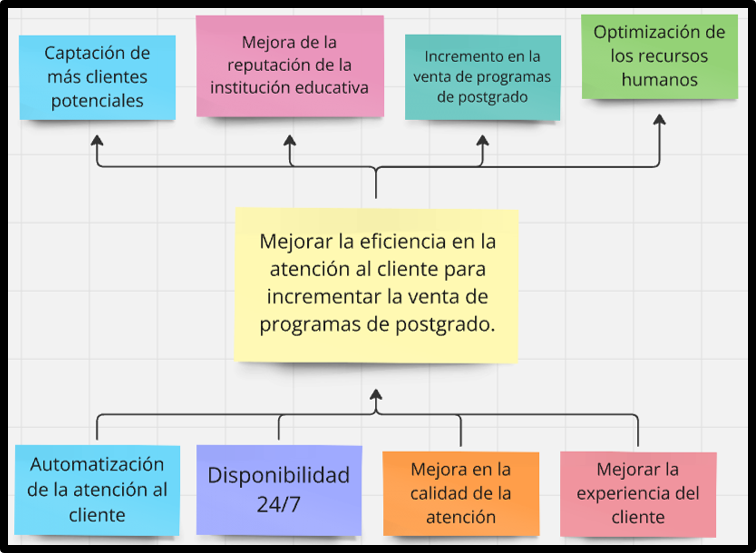
\includegraphics[scale=0.80]{ArbolObjetivos.png} \hfill 
	\end{figure}
  
%%%%%%%%%%%%%%%%%%%%%%%%%%%%%%%%%%%%%%%%%%%%%%%%%%%%%%%%%%%%%%%%%%%%%%%%%%

    \subsection{Matriz de Consistencia} 
	
	\begin{figure}[H]
		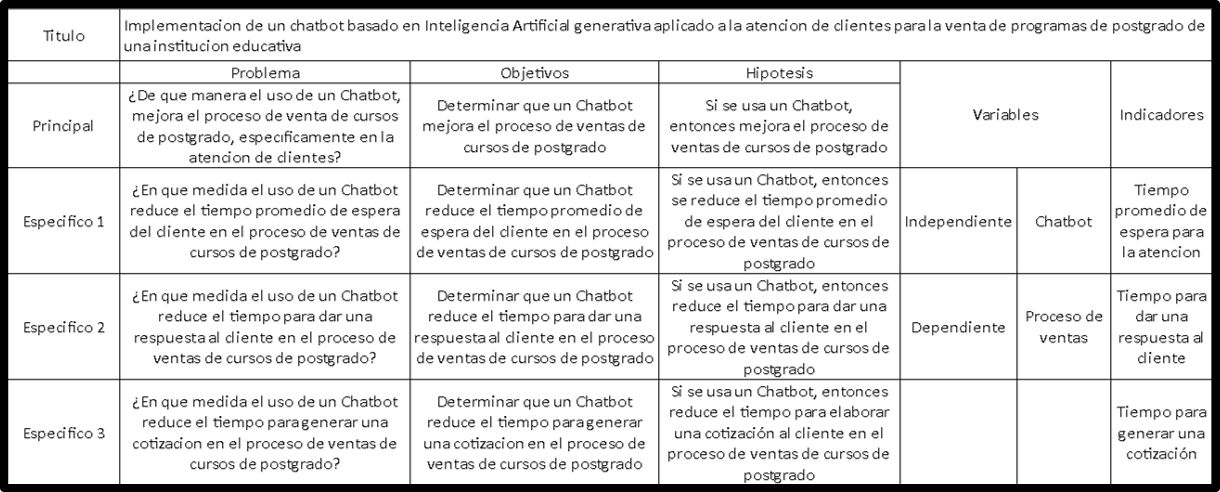
\includegraphics[scale=0.5]{MatrizConsistencia.png} \hfill 
	\end{figure}
	
\end{document}

